\section{Water Models}\label{sec:water_models}

% Navier stokes, Different level of water depth, Spatial, Spectral domain,
% eulerian, lagrangian frameworks, talk about their visual accuracy, SLProject,
% 0 a.d.

% Talk about the different depth of water

In this section we start by presenting the physical accurate description of
fluids in \autoref{subsec:navier_stokes}. Then in
\autoref{subsec:spatial_domain} and \autoref{subsec:spectral_domain} we describe
the two existing groups of water models appearing the literature: spatial and
spectral.  For each of them we selected a couple of relevant approaches that
will be explained. Finally in \autoref{subsec:candidate_apps} we present two
applications which need a real-time water solution.

\subsection{Navier-Stokes Equations}\label{subsec:navier_stokes}

% explain that they describe a fluid but they don't have a solution yet and it's
% one of the biggest open problems in math. Computational Fluid Dynamics CFD is
% the field of finding numerical approximations to the equations
% The process of solving problems in fluid dynamics numerically on a computer is
% called CFD


\subsection{Spatial Domain}\label{subsec:spatial_domain}

% What is the spatial domain?
% present some papers:
% - Johanson

\subsection{Spectral Domain}\label{subsec:spectral_domain}

% What is the spectral domain?

% present some models in the spectral and spatial domains from different papers
% that look great:
% - Tessendorf


\subsection{Methods Used in Industry Productions}\label{subsec:methods_industry}

% FFT, Projected Grid, LOD, talk about world of warships, anno, and oceans on a
% shoestring and uncharted. Talk also about some available shaders in the Unity
% store, the default one in Unity, and in Unreal Engine, also in Cryengine.

Many different water models are used in industry productions. One that has been
applied extensively in movies and most of the games is the one from
Tessendorf \autocite{tessendorf2001simulating} as seen
in \autoref{subsec:spectral_domain}. During our research we came across three
solutions which where presented at the Game Developer Conference or at the
SIGGRAPH conference. They are implemented in Uncharted, World of Warships and an
undisclosed game.



\subsection{Candidate Applications for Embedding}\label{subsec:candidate_apps}

We now present two candidate applications which need a real-time water model:
\textit{SLProject} and \textit{0 A.D.}. Although both have already one,
in the former application the model doesn't work and in the latter it is
outdated.


\subsubsection{SLProject}

\textit{SLProject} is a Scene Library developed and maintained by the cpvrLab at
the Bern University of Applied Sciences (BFH). It is free and open
source\footnote{Licensed under the GNU-GPL license.} and runs on Windows, MacOS,
Linux, Android and iOS\@. The project is a showcase for 3D computer graphics and
image processing topics such as real-time rendering, raytracing and feature
tracking. It is coded in C++ and OpenGL ES to ensure complete platform
independence \autocite{hudritch2017slproject, slproject2017doxygen}.

The project has a real-time water rendering demo but it is unfortunately broken
(see open ticket, \#36 ``Fix water
shader''\footnote{\url{https://github.com/cpvrlab/SLProject/issues/36}}). The
water plane is modeled by a simple multiplication of the sine and cosine
functions and is illuminated 50\% by a point light and 50\% by a cube texture.


\subsubsection{0 A.D.}

\textit{0 A.D.} is a real-time strategy game representing the 500 B.C to 500 A.D
era. It is developed by Wildfire Games, an independent game development studio.
The game is free, open source\footnote{Licensed under the GNU-GPL and CC BY-SA
license.} and runs on Windows, MacOS and Linux.

The development of the game began in 2000 when three modding groups whished to
create a free game engine. Up until 2009 the source code was accessible only to
members of Wildfire Games. Anyone interested in participating could make an
application and pass an interview. However, due to the fading interest of a
mod\footnote{Shorthand for the term \textit{modification}} which used 0 A.D.'s
game engine and the lack of programmers, they opened up the code in July 2009.
From then on many contributions have been made, notably one redesigning entirely
the code base, making new contributions easier. As of today the project is still
actively maintained, with the latest alpha-release (number 22 code named
``Venustas'') dating from July 26,
2017 \autocite{wildfire0adproject,wildfire0adstory}.

The game engine, Pyrogenesis, is heavily oriented towards modding. The core
engine is coded in C++ and Javascript is used for the game's logic, like the
artificial intelligence or the random generation of maps. This means that when
\textit{0 A.D.} is run the game engine is started with a given mod. A mod
contains all the graphical elements, 3D models, sound, shaders, scenarios, map
generators and artificial intelligence.

The documentation for developers provides good build instructions, coding
conventions and codebase descriptions. Unfortunately we found that it is
difficult for a newcomer to understand the game engine architecture. It is less
documented and scattered accross multiple pages which are sometimes outadated.
The Doxygen documentation is minimalistic and unlike the one from
\textit{SLProject}, does not help to understand the architecture.

The current water implementation has been created in 2006 by a student form the
University of Waterloo, Canada, as a course project \autocite{zaharia2006cs}.
Over the years it has been slightly modified and optimized but appears visually
outdated (see \autoref{fig:0ad_water} on page~\pageref{fig:0ad_water}) compared
to the one used in commercial RTS games like Anno 1800 or Age of Empires~3
\todo[inline]{reference figure from introduction}. There is an open ticket, \#48
``Advanced Water
Rendering''\footnote{\url{https://trac.wildfiregames.com/ticket/48}}, which was
opened twelve years ago and modified three years ago but still not closed.  We
have contacted the developers and they would gladly appreciate a contribution
that would close the issue.

\begin{figure}[t!]
    \centering
    \begin{subfigure}[t]{\textwidth}
        \centering
        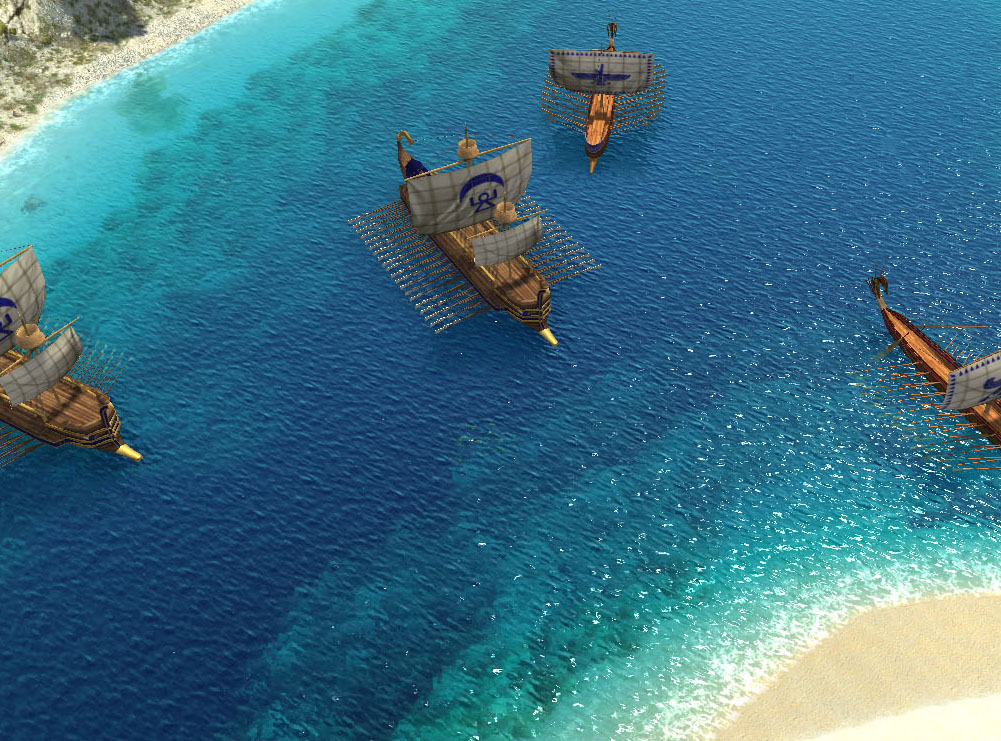
\includegraphics[height=5cm]{figures/0ad_water-specular.jpg}
        \subcaption{Close view of the water.}\label{subfig:0ad_water_close}
    \end{subfigure}\\%
    %  
    \begin{subfigure}[t]{\textwidth}
        \centering
        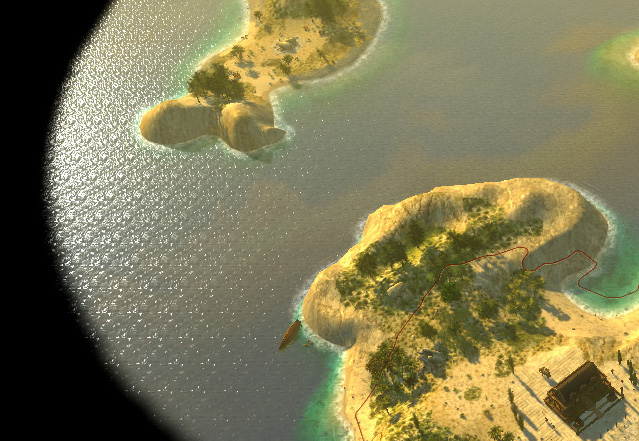
\includegraphics[height=5cm]{figures/0ad_cycladic_arcgipelago_6.jpg}
        \subcaption{Zoomed out view.}\label{subfig:0ad_water_far}
    \end{subfigure}
    \caption{\textit{0 A.D.}'s water rendering. Notice on the lower left part
        of \autoref{subfig:0ad_water_close} the repetition of the waves.
        In \autoref{subfig:0ad_water_far} it is even more apparent (source:
        \url{play0ad.com}).}\label{fig:0ad_water}
\end{figure}
